\documentclass[12pt]{article}
\usepackage{graphicx,import}
\usepackage[svgnames]{xcolor} 
\usepackage{fancyhdr}
\usepackage{subfig}
\usepackage{hyperref}
\usepackage{enumitem}
\usepackage[many]{tcolorbox}
\usepackage{listings}
\usepackage[a4paper, total={6in, 8in} , bottom = 25mm , top = 25mm, headheight = 1.25cm , includehead,includefoot,heightrounded ]{geometry}
\usepackage{afterpage}
\usepackage{amssymb}
\usepackage{pdflscape}
\usepackage{gensymb}
\usepackage{textcomp}
\usepackage{tikz,pgfplots}
\usepackage{xecolor}
\usepackage{rotating}
\usepackage{pdfpages}
\usepackage[T1]{fontenc}
\usepackage{tikz}
\usepackage[utf8]{inputenc}
\usepackage{PTSerif} 
\usepackage{seqsplit}
\usepackage{fancyvrb}
\usepackage{mips}
\usepackage{multirow}
\usepackage{hhline}
\usepackage[edges]{forest}
\usepackage{tabularx}
\usepackage{float}
\usepackage{graphicx}
\usepackage{cprotect}
\usepackage{url}
\usepackage{listings}
\usepackage{xcolor}
\usepackage{pifont}
\newcommand{\xmark}{\ding{55}}%
\def\checkmark{\tikz\fill[scale=0.4](0,.35) -- (.25,0) -- (1,.7) -- (.25,.15) -- cycle;}

\hypersetup{
	colorlinks   = true, %Colours links instead of ugly boxes
	urlcolor     = blue, %Colour for external hyperlinks
	linkcolor    = blue, %Colour of internal links
	citecolor   = red %Colour of citations
}

\definecolor{codegreen}{rgb}{0,0.6,0}
\definecolor{codegray}{rgb}{0.5,0.5,0.5}
\definecolor{codepurple}{rgb}{0.58,0,0.82}
\definecolor{backcolour}{rgb}{0.95,0.95,0.92}
\definecolor{mGreen}{rgb}{0,0.6,0}
\definecolor{mGray}{rgb}{0.5,0.5,0.5}
\definecolor{mPurple}{rgb}{0.58,0,0.82}
\definecolor{backgroundColour}{rgb}{0.95,0.95,0.92}

\NewDocumentCommand{\codeword}{v}{
	\texttt{\textcolor{blue}{#1}}
}
\lstset{language=java,keywordstyle={\bfseries \color{blue}}}
\definecolor{dkgreen}{rgb}{0,0.6,0}
\definecolor{gray}{rgb}{0.5,0.5,0.5}
\definecolor{mauve}{rgb}{0.58,0,0.82}



\lstdefinestyle{mystyle}{
	backgroundcolor=\color{backcolour},   
	commentstyle=\color{codegreen},
	keywordstyle=\color{magenta},
	numberstyle=\tiny\color{codegray},
	stringstyle=\color{codepurple},
	basicstyle=\ttfamily\normalsize,
	breakatwhitespace=false,         
	breaklines=true,                 
	captionpos=b,                    
	keepspaces=true,                 
	numbers=left,                    
	numbersep=5pt,                  
	showspaces=false,                
	showstringspaces=false,
	showtabs=false,                  
	tabsize=2
}

\lstdefinestyle{CStyle}{
	backgroundcolor=\color{backgroundColour},   
	commentstyle=\color{mGreen},
	keywordstyle=\color{magenta},
	numberstyle=\tiny\color{mGray},
	stringstyle=\color{mPurple},
	basicstyle=\footnotesize,
	breakatwhitespace=false,         
	breaklines=true,                 
	captionpos=b,                    
	keepspaces=true,                 
	numbers=left,                    
	numbersep=5pt,                  
	showspaces=false,                
	showstringspaces=false,
	showtabs=false,                  
	tabsize=2,
	language=C
}



\lstset{ %
	language=[mips]Assembler,       % the language of the code
	basicstyle=\footnotesize,       % the size of the fonts that are used for the code
	numbers=left,                   % where to put the line-numbers
	numberstyle=\tiny\color{gray},  % the style that is used for the line-numbers
	stepnumber=1,                   % the step between two line-numbers. If it's 1, each line
	% will be numbered
	numbersep=5pt,                  % how far the line-numbers are from the code
	backgroundcolor=\color{white},  % choose the background color. You must add \usepackage{color}
	showspaces=false,               % show spaces adding particular underscores
	showstringspaces=false,         % underline spaces within strings
	showtabs=false,                 % show tabs within strings adding particular underscores
	frame=single,                   % adds a frame around the code
	rulecolor=\color{black},        % if not set, the frame-color may be changed on line-breaks within not-black text (e.g. commens (green here))
	tabsize=4,                      % sets default tabsize to 2 spaces
	breaklines=true,                % sets automatic line breaking
	breakatwhitespace=false,        % sets if automatic breaks should only happen at whitespace
	% also try caption instead of title
	keywordstyle=\color{blue},          % keyword style
	commentstyle=\color{dkgreen},       % comment style
	stringstyle=\color{mauve},         % string literal style
	escapeinside={\%*}{*)},            % if you want to add a comment within your code
	morekeywords={*,...}               % if you want to add more keywords to the set
}

\setmainfont[ExternalLocation=fonts/]{EBGaramond-Regular.ttf}




\newenvironment{changemargin}[2]{%
	\begin{list}{}{%
			\setlength{\topsep}{0pt}%
			\setlength{\leftmargin}{#1}%
			\setlength{\rightmargin}{#2}%
			\setlength{\listparindent}{\parindent}%
			\setlength{\itemindent}{\parindent}%
			\setlength{\parsep}{\parskip}%
		}%
		\item[]}{\end{list}}


\definecolor{foldercolor}{RGB}{124,166,198}

\tikzset{pics/folder/.style={code={%
			\node[inner sep=0pt, minimum size=#1](-foldericon){};
			\node[folder style, inner sep=0pt, minimum width=0.3*#1, minimum height=0.6*#1, above right, xshift=0.05*#1] at (-foldericon.west){};
			\node[folder style, inner sep=0pt, minimum size=#1] at (-foldericon.center){};}
	},
	pics/folder/.default={20pt},
	folder style/.style={draw=foldercolor!80!black,top color=foldercolor!40,bottom color=foldercolor}
}

\forestset{is file/.style={edge path'/.expanded={%
			([xshift=\forestregister{folder indent}]!u.parent anchor) |- (.child anchor)},
		inner sep=1pt},
	this folder size/.style={edge path'/.expanded={%
			([xshift=\forestregister{folder indent}]!u.parent anchor) |- (.child anchor) pic[solid]{folder=#1}}, inner xsep=0.6*#1},
	folder tree indent/.style={before computing xy={l=#1}},
	folder icons/.style={folder, this folder size=#1, folder tree indent=3*#1},
	folder icons/.default={12pt},
}

\begin{document}
	
	
%%% title pages
\begin{titlepage}
	\begin{center}
		
		\vspace*{0.7cm}
		
		
\includegraphics[width=0.4\textwidth]{sharif1.png}\\
		\vspace{0.5cm}
		\textbf{ \Huge{Multicore Computing} }\\
		\vspace{0.5cm}
		\textbf{ \Large{ Assignment Three (Practical)} }
		\vspace{0.2cm}
		
		
		\large \textbf{Department of Computer Engineering}\\\vspace{0.2cm}
		\large   Sharif University of Technology\\\vspace{0.2cm}
		\large   Spring 2022 \\\vspace{0.2cm}
		\noindent\rule[1ex]{\linewidth}{1pt}
		Lecturer:\\
		\textbf{{Dr. Falahati}}
		
		
		\vspace{0.15cm}
		Name - Student Number:\\
		
		\textbf{{Saba Hashemi - 97100581}}\\
		
		\textbf{{Amirmahdi Namjoo - 97107212}}
	\end{center}
\end{titlepage}
%%% title pages


%%% header of pages
\newpage
\pagestyle{fancy}
\fancyhf{}
\fancyfoot{}
\cfoot{\thepage}
\chead{ Amirmahdi Namjoo - Saba Hashemi}
\rhead{
\includegraphics[width=0.1\textwidth]{sharif.png}}
\lhead{Assignment Three}
%%% header of pages



\section{Question One}

\begin{itemize}
	
	\item Team member No.1: Saba Hashemi,97100581
	\item Team member No.2: Amirmahdi Namjoo,97107212
\end{itemize}

\newpage

\section{Question Two}


\newpage

\section{Question Three}

Note: All parts are run on Intel Core i9 11980HK with 8 physical cores and 16 logical cores. The results on 16 threads may vary (and show less performance) on systems that have less than 16 logical cores.

\begin{enumerate}[label=\alph*.]
	\item 
	The code is included in \Verb+Q3.c+.
	
	\item 
	The results of running the code for different parameters are included in \Verb+results3.xlsx+. Note that it has multiple sheets and the name of each sheet represents the parameters given to the program. The column with title 1 shows the results of running the unparalleled version of the code. All other columns represent the results of running the Parallelized version of the code with OpenMP.

\item
Plots for different input parameters:

\begin{figure}[H]
	\centering
	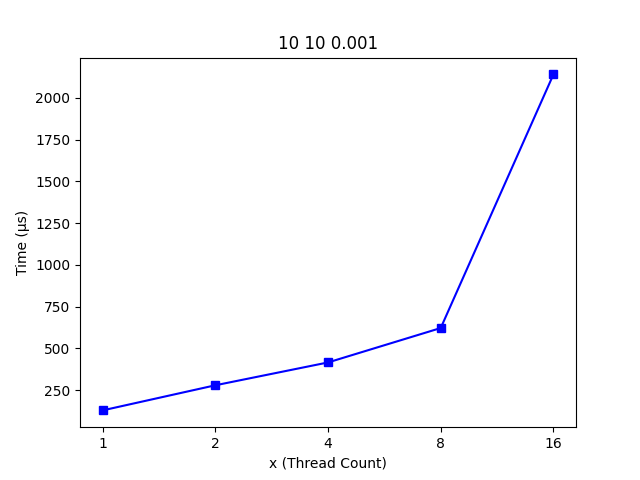
\includegraphics[width=0.5\textwidth]{./images/Q3/10100001.png}	
	\cprotect\caption{Results of running the code with parameters $10$ $10$ $0.001$}
	\label{fig:1}
\end{figure}

\begin{figure}[H]
	\centering
	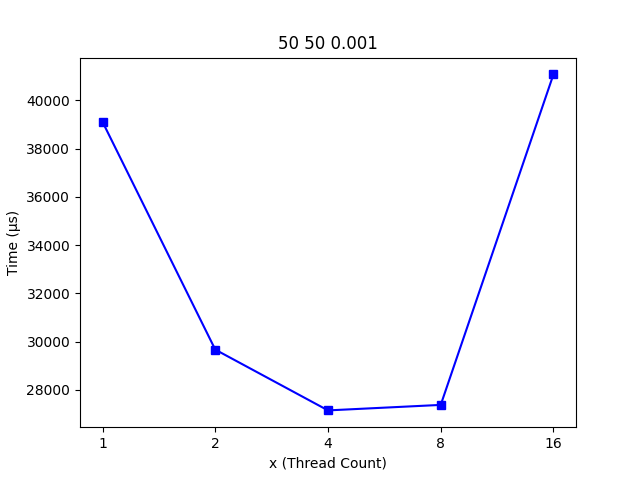
\includegraphics[width=0.5\textwidth]{./images/Q3/50500001.png}	
	\cprotect\caption{Results of running the code with parameters $50$ $50$ $0.001$}
	\label{fig:2}
\end{figure}

\begin{figure}[H]
	\centering
	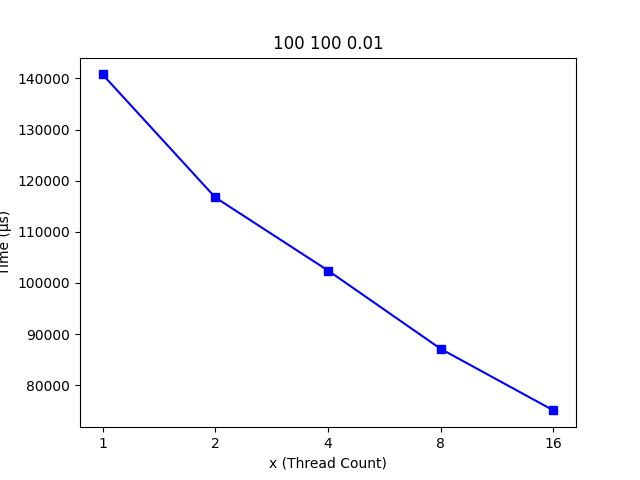
\includegraphics[width=0.5\textwidth]{./images/Q3/100100001.png}	
	\cprotect\caption{Results of running the code with parameters $100$ $100$ $0.01$}
	\label{fig:3}
\end{figure}


\begin{figure}[H]
	\centering
	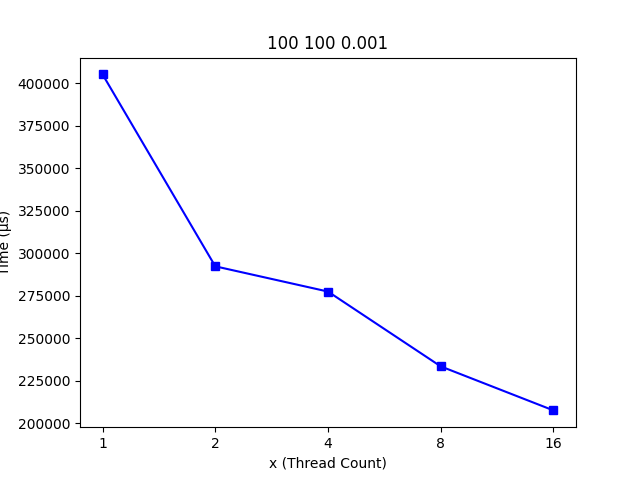
\includegraphics[width=0.5\textwidth]{./images/Q3/1001000001.png}	
	\cprotect\caption{Results of running the code with parameters $100$ $100$ $0.001$}
	\label{fig:4}
\end{figure}

\begin{figure}[H]
	\centering
	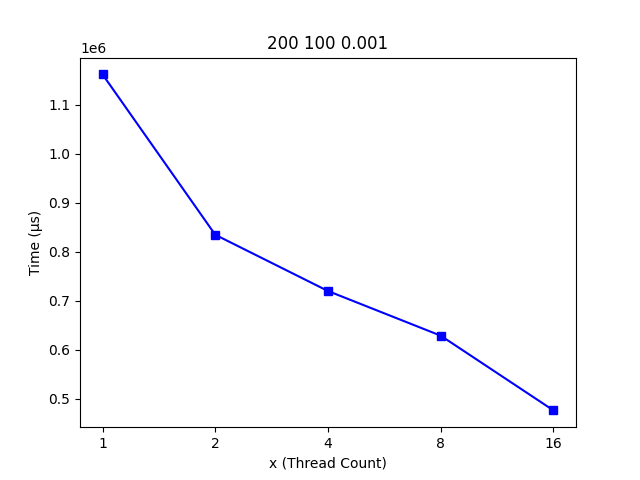
\includegraphics[width=0.5\textwidth]{./images/Q3/2001000001.png}	
	\cprotect\caption{Results of running the code with parameters $200$ $100$ $0.001$}
	\label{fig:5}
\end{figure}

\begin{figure}[H]
	\centering
	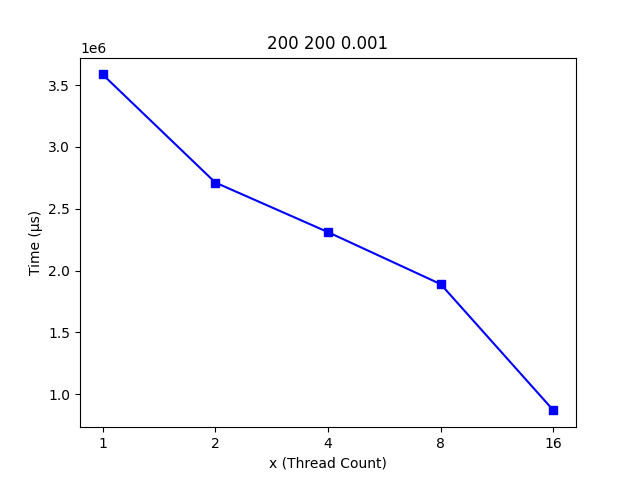
\includegraphics[width=0.5\textwidth]{./images/Q3/2002000001.png}	
	\cprotect\caption{Results of running the code with parameters $200$ $200$ $0.001$}
	\label{fig:6}
\end{figure}

\begin{figure}[H]
	\centering
	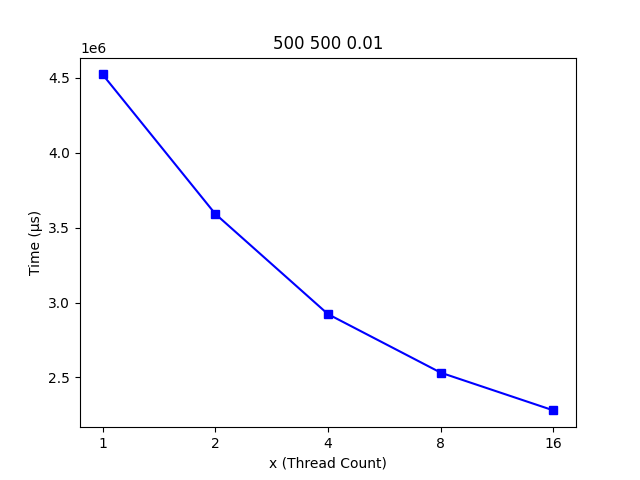
\includegraphics[width=0.5\textwidth]{./images/Q3/500500001.png}	
	\cprotect\caption{Results of running the code with parameters $500$ $500$ $0.01$}
	\label{fig:7}
\end{figure}


\item 
With very small inputs like $n=10,m=10$ (Figure \ref{fig:1}), we see that the overhead of creating new threads is too high that it causes the parallelized code to perform worse than the serial code.

For medium inputs like $n=50,m=50$ (Figure \ref{fig:2}), we see that at first, parallelization has a positive effect. Still, after increasing the number of threads from 8 to 16, the overhead of creating new threads overcomes the positive effects of parallelization.

For $n=100, m=100$, we see an increase in performance by increasing the thread count. Notably, this improvement rate decreases after a while; it is evident in Figure \ref{fig:4}. Also, by comparing Figure \ref{fig:3} and Figure \ref{fig:4}, we can find out that decreasing the tolerance decreases the overall runtime of the program (as expected). This decrease in overall runtime causes the positive effect of parallelization in Figure \ref{fig:3} to pale compared to Figure \ref{fig:4}.

For larger inputs like $n=200, m=200$ (Figure \ref{fig:6}) and $n=500, m=500$ (Figure \ref{fig:7}), we see similar results; i.e. The parallelization has a positive effect. Also, except for the last entry in Figure \ref{fig:6}, we see the rate of this improvement decreases by increasing the number of threads. The exception for the last entry of Figure \ref{fig:6} is maybe caused by $200\times200$ being divisible by $64$ and this divisibility by a large power of two caused the $16$ thread version to perform better on this case.

 
\end{enumerate}

\newpage

\section{Question Four}

Note: All parts are run on Intel Core i9 11980HK with 8 physical cores and 16 logical cores. The results on 16 threads may vary (and show less performance) on systems that have less than 16 logical cores.

\begin{enumerate}[label=\alph*.]
	
	\item 
		The code is included in \Verb+Q4.c+.
	
	\item 
		The code is included in \Verb+Q4_Parallel.c+.
		
	\item 
	You can find the raw results for runtime (in $\micro s$) in \Verb+results4.xlsx+. The plot is shown in Figure \ref{fig:8}. We run the the code for $N=8$ to $N=16$. After that, the amount of time needed to execute was very high, and it was not feasible to continue. We tested each case for thread counts of $1,4,8,16$. Note that the y-axis is shown in logarithmic scale (base $10$).
	
	
	\begin{figure}[H]
		\centering
		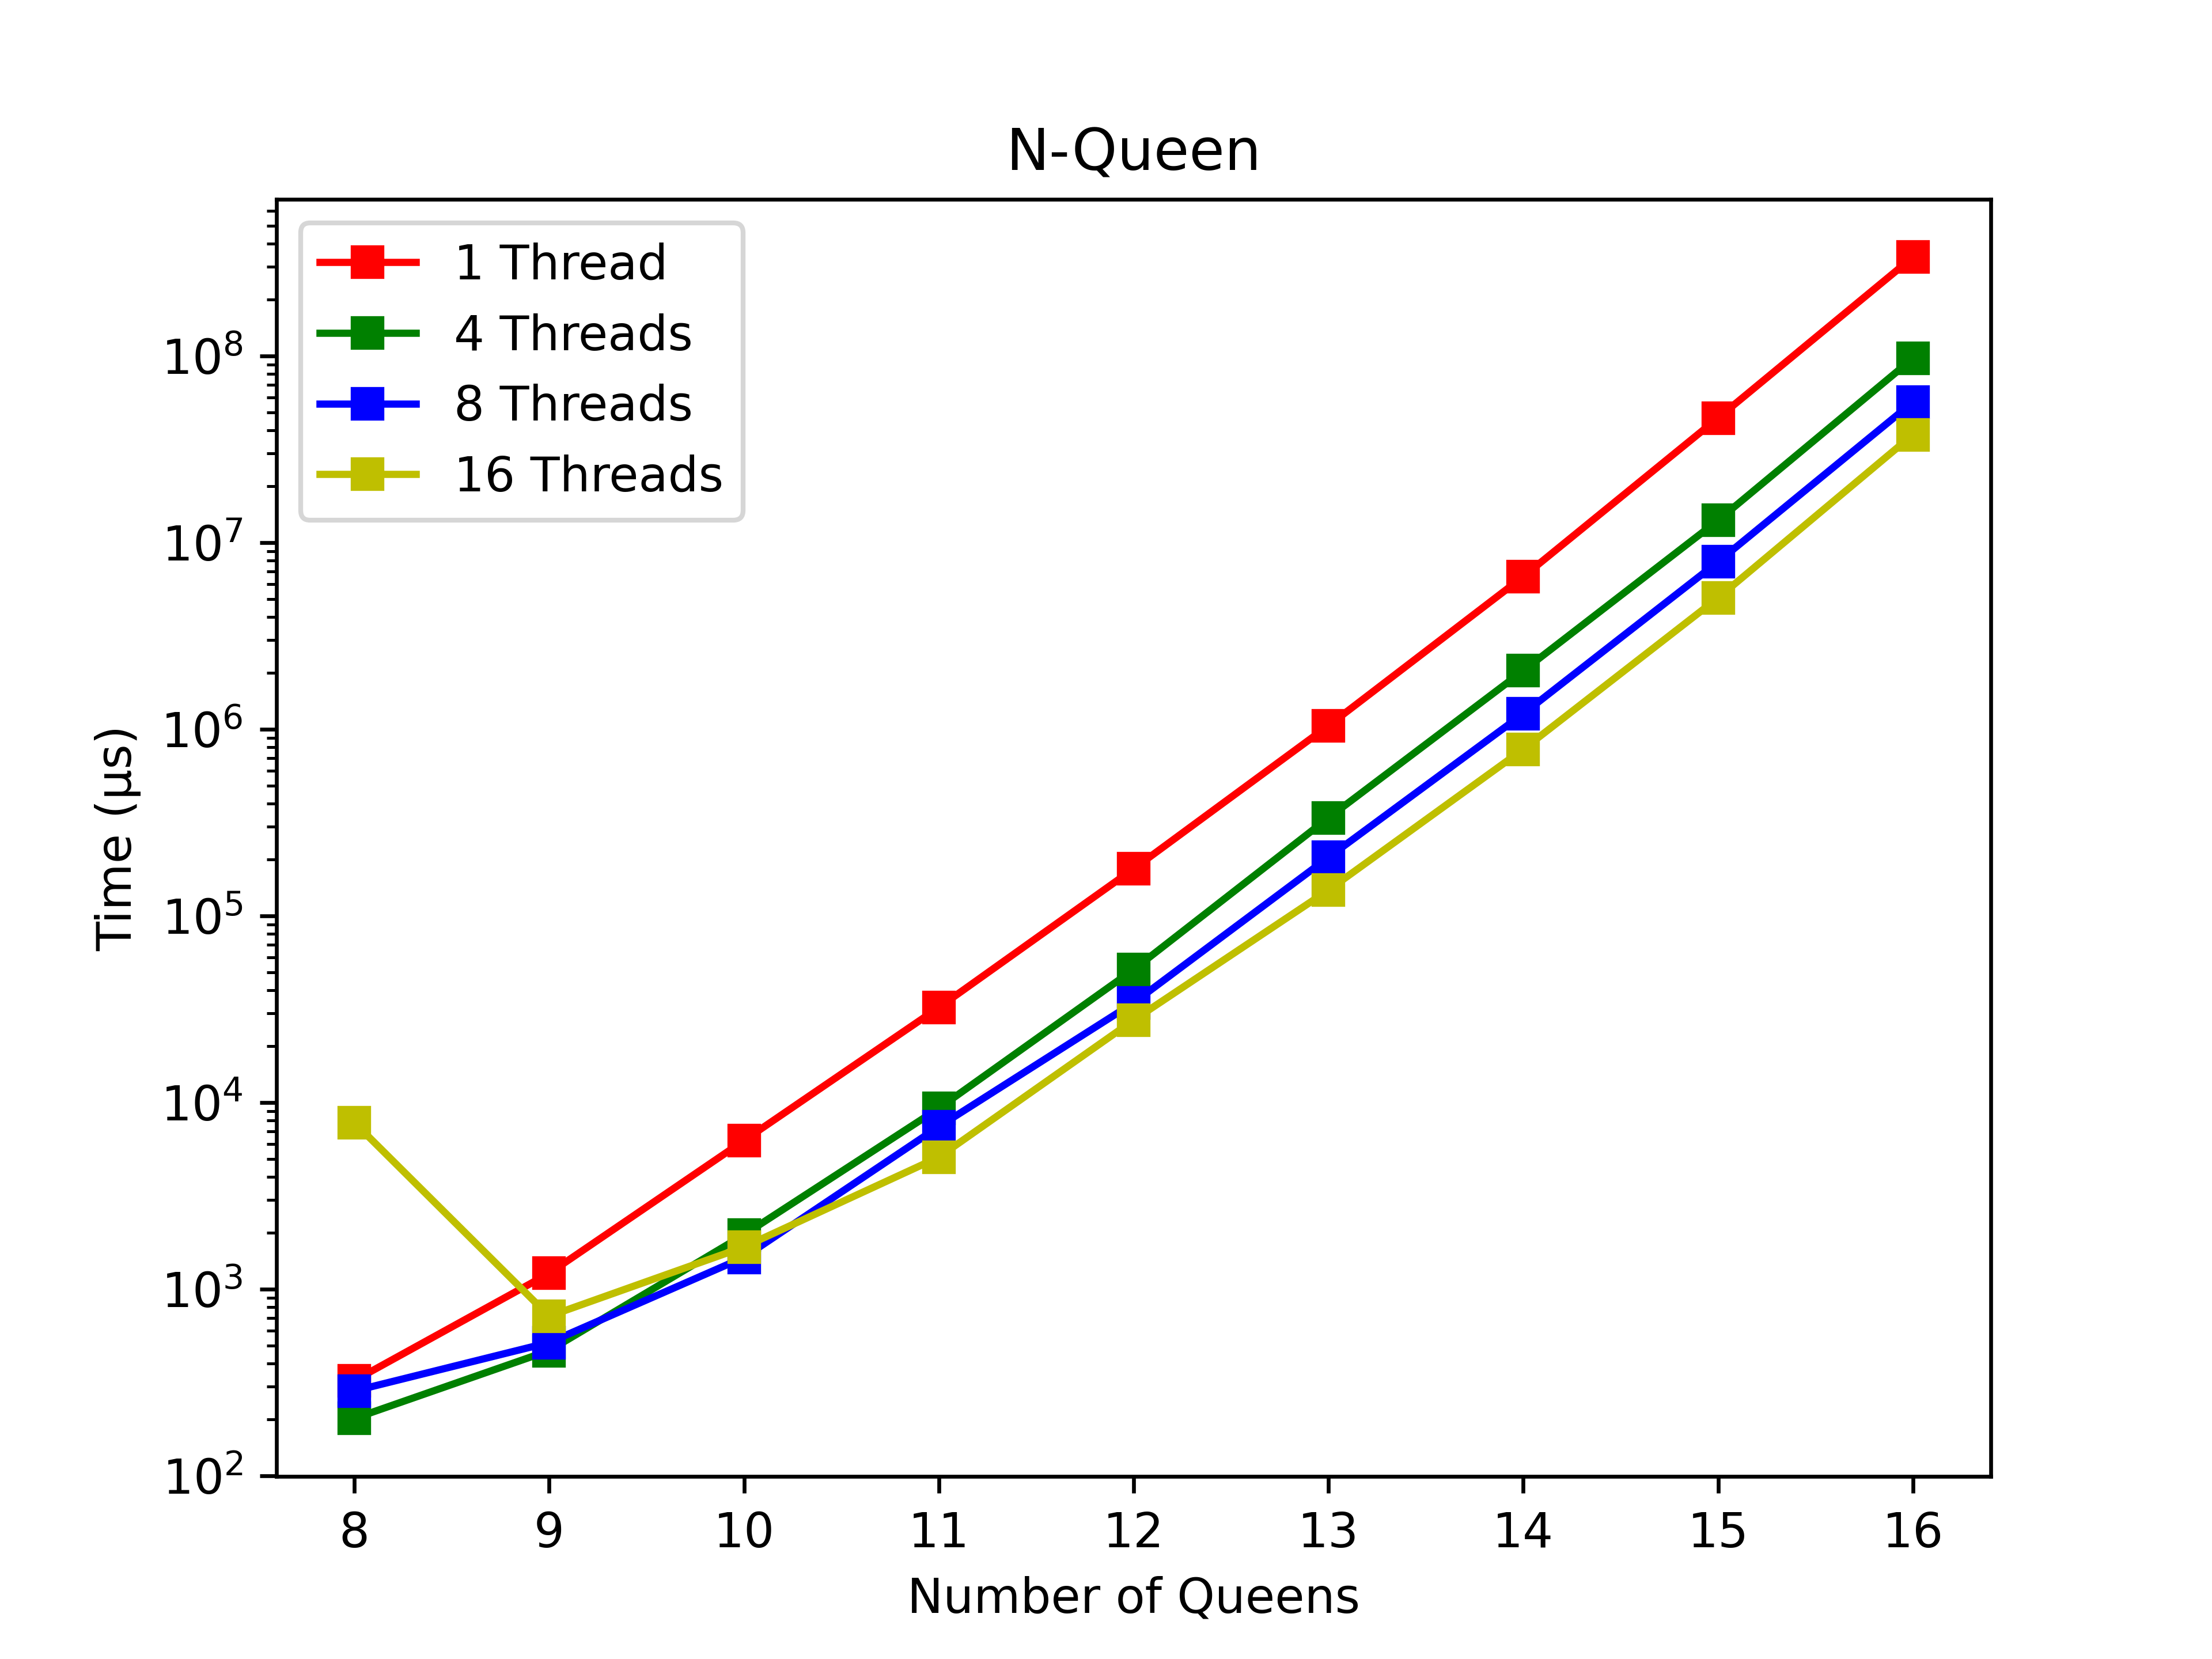
\includegraphics[width=0.5\textwidth]{./images/Q4/N-Queen.png}	
		\cprotect\caption{Results of running the N-Queen code for $N=8$ to $N=16$ and thread counts of $1,4,8,16$}
		\label{fig:8}
	\end{figure}
	
	
	\item 
	Yes. We got a performance boost. We used \Verb+task+ construct in OpenMP. which actually puts the function specified in a queue so that each free thread picks up one task and executes it from the queue.

	For the first cases like $N=8$, $N=9$, and $N=10$, the overhead of creating $16$ threads was too high, and it performed worse than the other cases; But for $N>11$, the $16$ threaded version performed better. 
	
	The linear shape of the plot on a logarithmic scale is also noteworthy. It shows that the growth rate of the running time is exponential.
	
	
\end{enumerate}

\newpage


\end{document}



